% Workshop wiskunde,  Jeroen Zuiddam

% beamer
\documentclass{beamer}
\mode<presentation>

% packages
\usepackage{amsmath,amssymb, amsfonts,mathrsfs}
\usepackage[dutch]{babel}
%\usepackage{hyperref}
\usepackage{graphicx}
%\usepackage{tikz}
%\usepackage{pgfplots}
%\usetikzlibrary{arrows}
%\usetikzlibrary{positioning}
%\usepackage{stmaryrd}
\usepackage{listings}
\usetheme{Watergraafsmeer}

\usepackage{enumerate}

% For every picture that defines or uses external nodes, you'll have to
% apply the 'remember picture' style. To avoid some typing, we'll apply
% the style to all pictures.
%\tikzstyle{every picture}+=[remember picture]

% front stuff
\author{Joris Stork, Jeroen Zuiddam en Lucas Swartsenburg}
\title{Kinect: hoe werkt het?}
\date{}

\begin{document}

\lstset{ %
language=Python,                % the language of the code
basicstyle=\footnotesize,       % the size of the fonts that are used for the code
backgroundcolor=\color{white},  % choose the background color. You must add \usepackage{color}
showspaces=false,               % show spaces adding particular underscores
showstringspaces=false,         % underline spaces within strings
showtabs=false,                 % show tabs within strings adding particular underscores
frame=single,                   % adds a frame around the code
tabsize=2,                      % sets default tabsize to 2 spaces
captionpos=b,                   % sets the caption-position to bottom
breaklines=true,                % sets automatic line breaking
breakatwhitespace=false,        % sets if automatic breaks should only happen at whitespace
}



\section{Introductie}
%% frame %%
\setbeamercolor{headline}{parent=white}
\begin{frame}
\titlepage
\end{frame}
\setbeamercolor*{headline}{parent=palette primary}

\begin{frame}{Kinect}{}
\centerline{
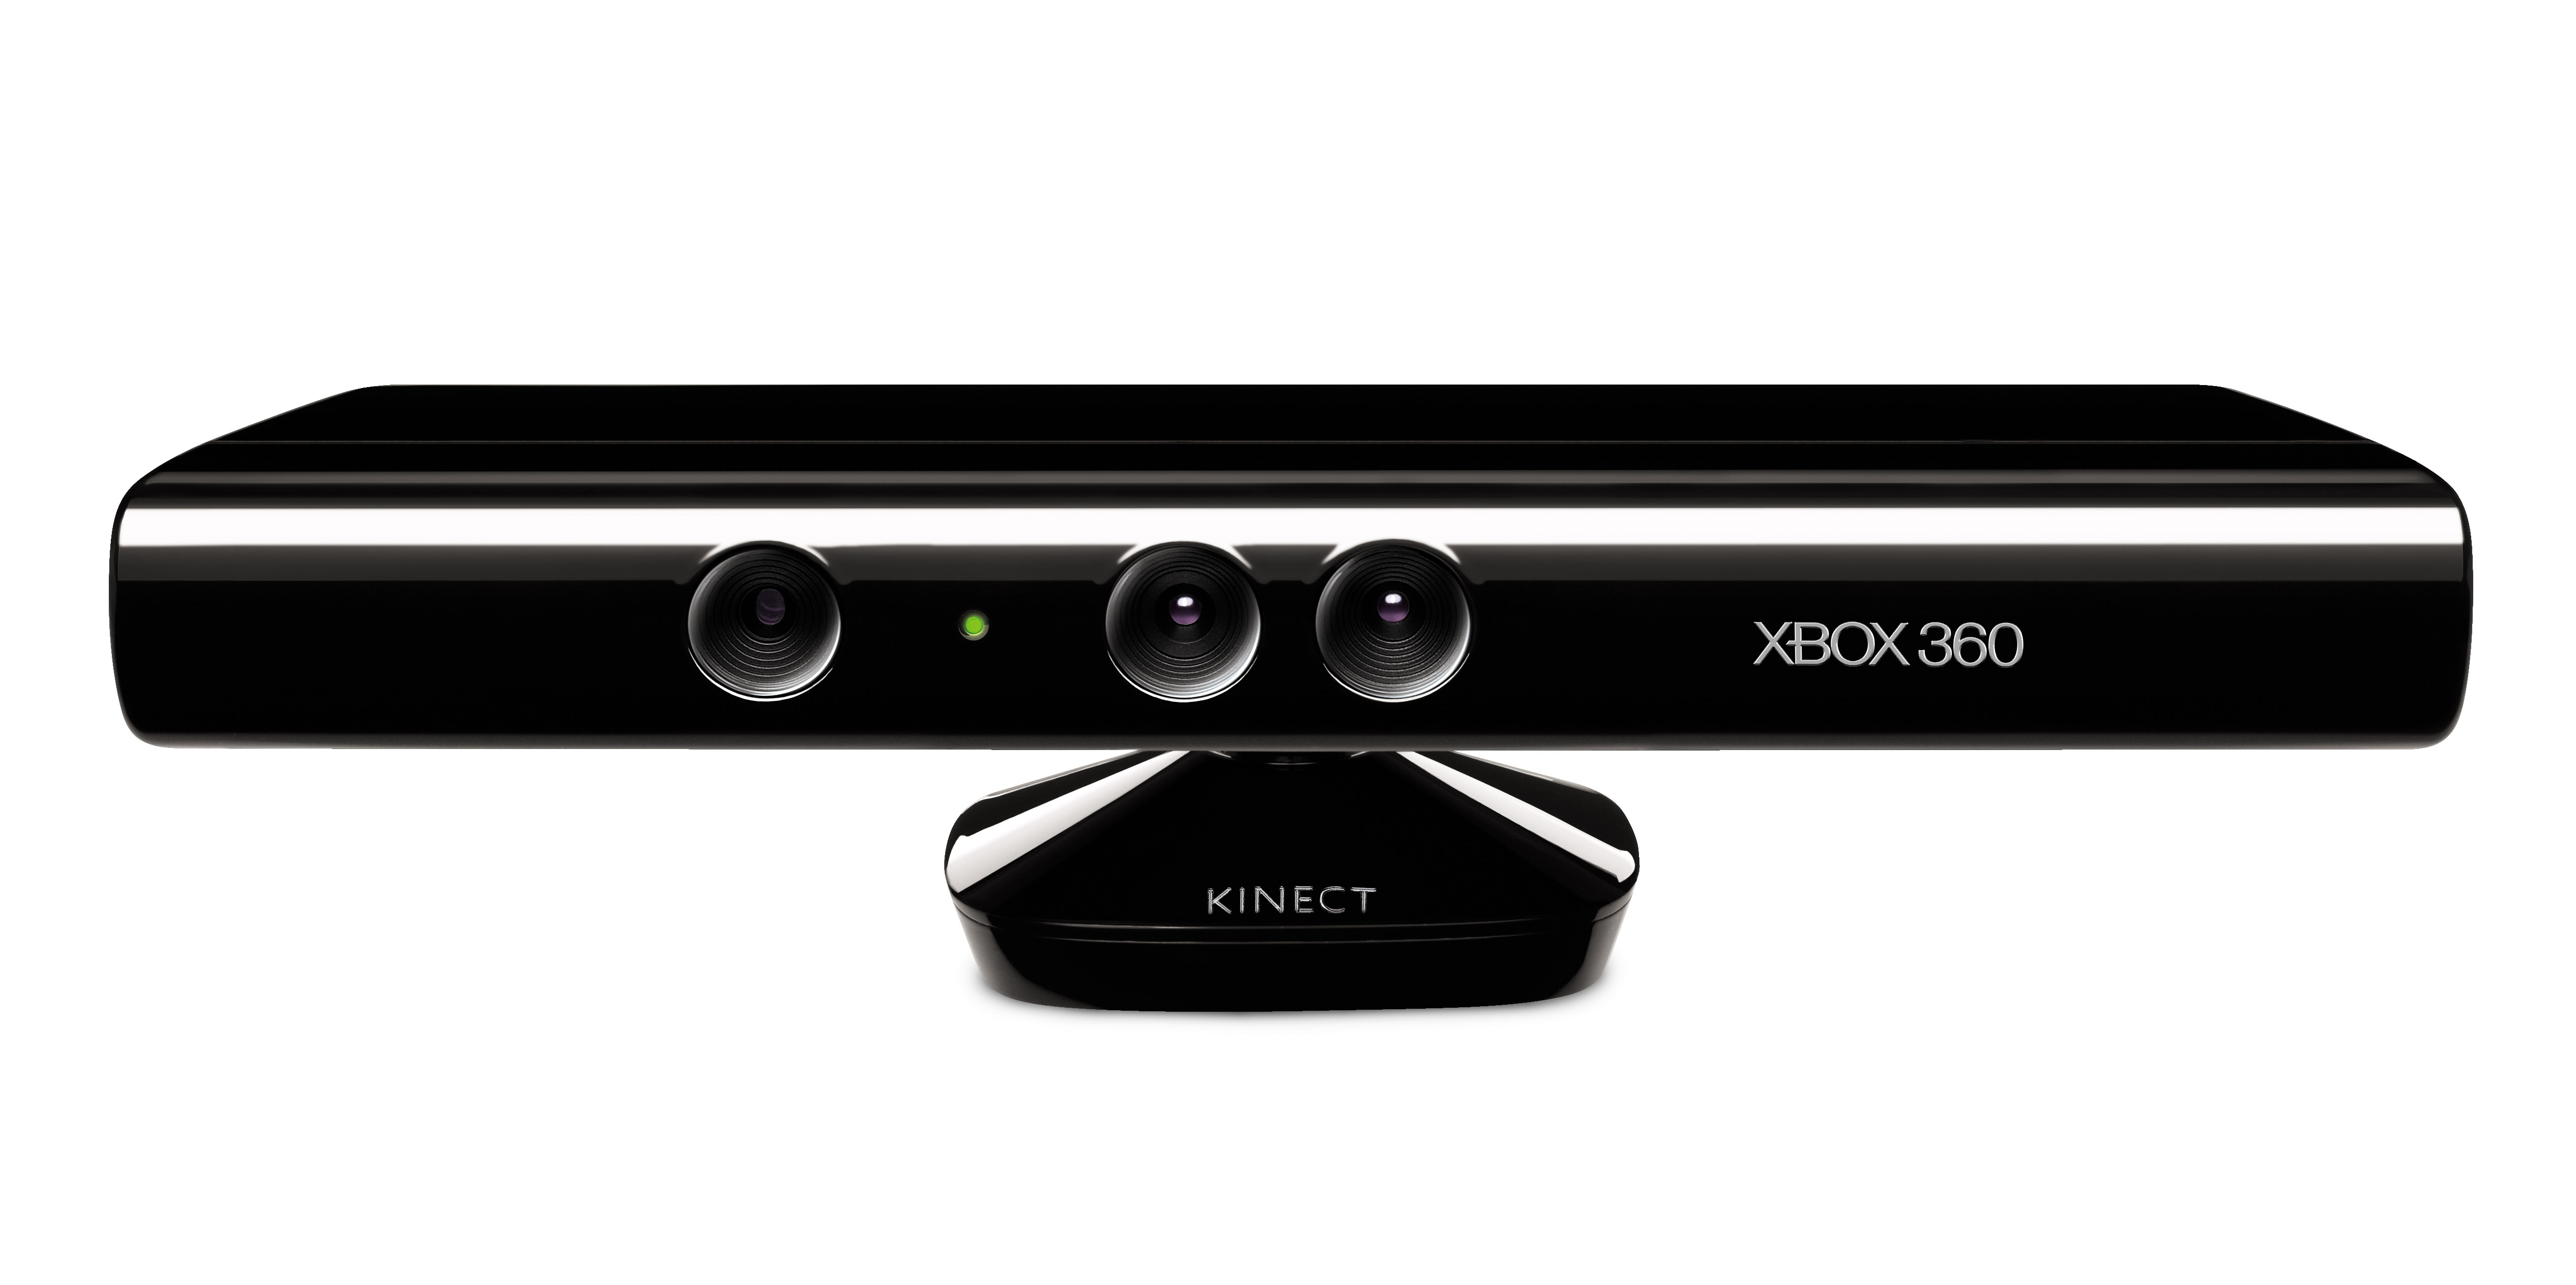
\includegraphics[scale=0.3, viewport= 40 120 1190 460, clip=true]{kinect.jpg}
}

\pause
\vfill
Vandaag beginnen we met: \\
\begin{columns}
\column{.25\textwidth}
\begin{enumerate}
\item \alt<3->{\textbf{correspondence}}{correspondence}
\item applicatie
\end{enumerate}
\pause
\column{.5\textwidth}
\begin{enumerate}
\item \textbf{Mellin transformatie}
\item \textbf{light coding}
\item \textbf{schaal identificatie}
\item \textbf{extra referentie beelden}
\end{enumerate}
\end{columns}
\end{frame}

\begin{frame}{Kinect}{}
\centerline{
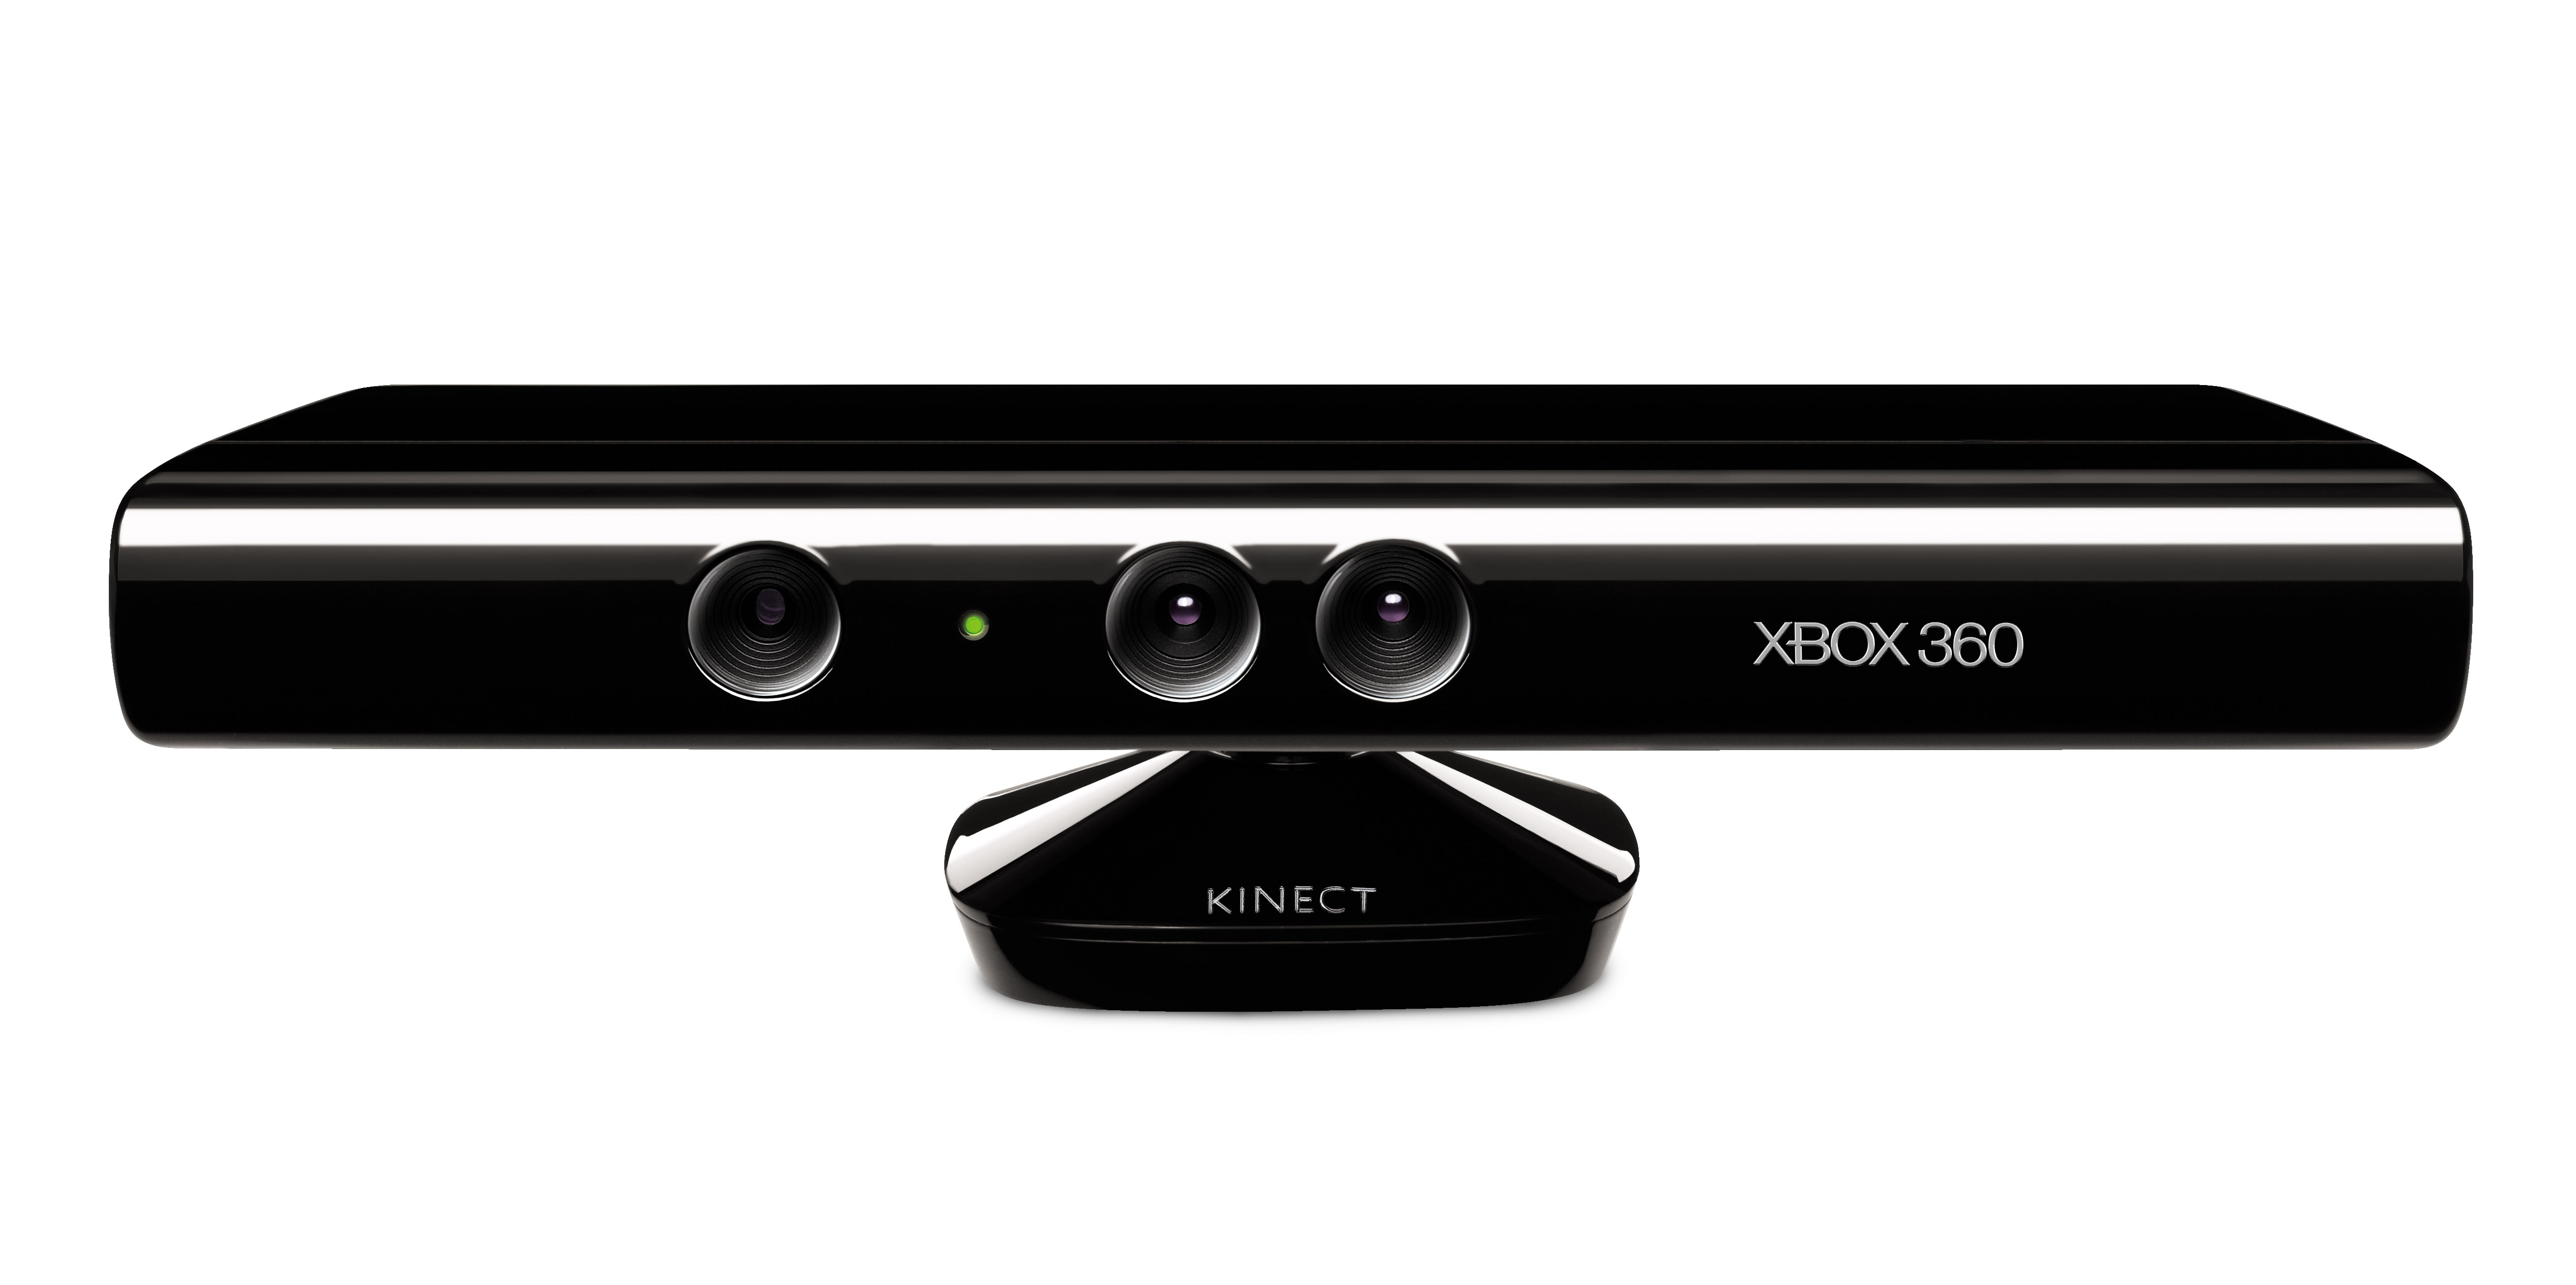
\includegraphics[scale=0.3, viewport= 40 120 1190 460, clip=true]{kinect.jpg}
}
\vfill
Daarna:\\
\begin{columns}
\column{.25\textwidth}
\begin{enumerate}
\item correspondence
\item \textbf{applicatie}
\end{enumerate}
\column{.5\textwidth}
\begin{enumerate}
\item \textbf{stereo calibratie}
\item \textbf{creating a model}
\item \textbf{point cloud viewer}
\end{enumerate}
\end{columns}
\end{frame}

\section{Werking}
\begin{frame}{Stereotriangulatie}

{\large Algemene situatie: twee willekeurige camera's}

\centerline{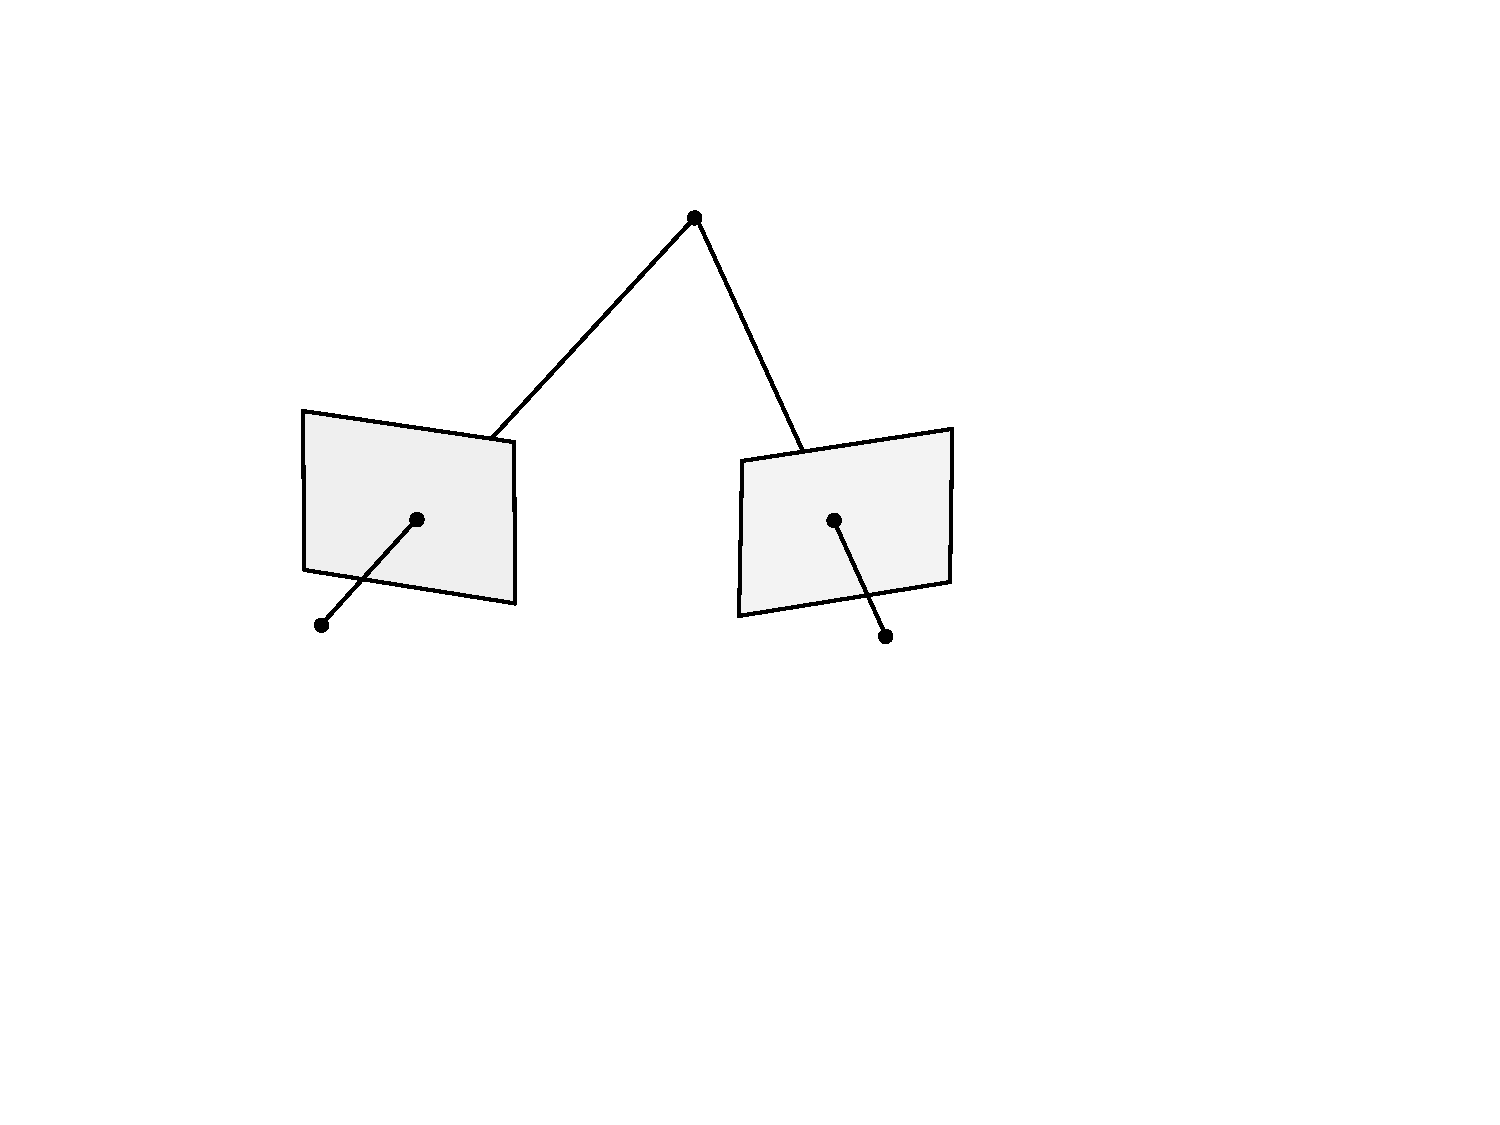
\includegraphics[scale=0.4, clip=true, viewport= 120 230 470 470]{triang}}
\vfill
\pause
{\large Rekenvoorbeeld: twee parallele pinhole cameras}
\pause
$$
\frac{z_1}{b} = \frac{z_1 - f}{b-x_l+x_r}\quad \pause\implies\quad z_1 = \frac {bf} {x_l - x_r}
$$
\end{frame}

\begin{frame}{Actieve stereotriangulatie}{}
{\large Algemene situatie}
\begin{enumerate}
\item camera
\item projector, laser of lamp
\end{enumerate}
\vfill
\pause
\centerline{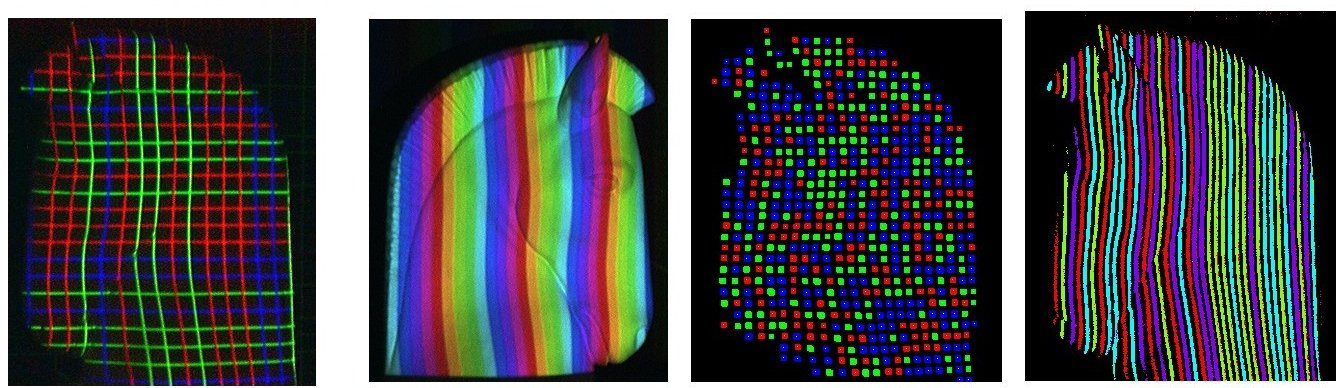
\includegraphics[scale=0.17]{structuredlight.jpg}\, 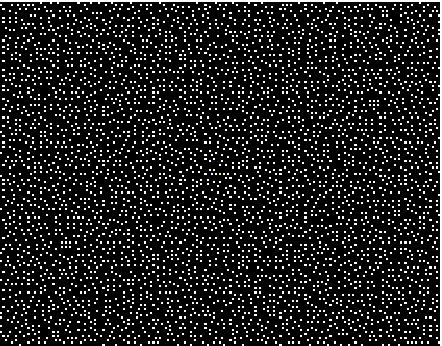
\includegraphics[scale=1, clip=true, viewport= 0 0 80 63]{kinect-pattern}}
\vfill
\pause
{\large Rekenvoorbeeld: `Kinect' met \'e\'en geprojecteerd punt}
\pause
$$
z_1 = \frac {z_0bf}{bf + r_0d}
$$
\end{frame}

\begin{frame}{Actieve stereotriangulatie}\vspace{-4pt}
\centerline{\includegraphics[scale=0.15, viewport=50 0 2700 1800, clip=true]{kinect_speckle.jpg}}
\end{frame}

%\begin{frame}{Actieve stereotriangulatie}\vspace{-4pt}
%\centerline{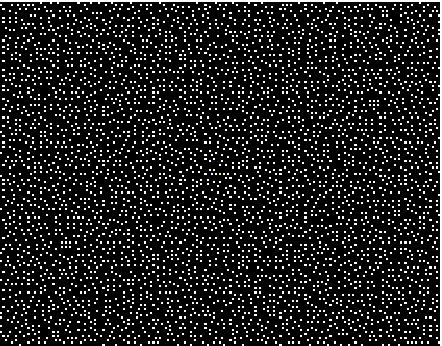
\includegraphics[scale=1.3]{kinect-pattern}}
%\end{frame}

\begin{frame}{Correspondence problem}

\begin{block}{Correspondence problem}
Welke referentiepunt hoort bij mijn punt?
\end{block}
\vfill
\pause
{\large Een oplossing}
\begin{columns}[t]
\column{.6\textwidth}
\begin{enumerate}
\item<+-> maak referentiebeelden
\item<+-> neem camerabeeld
\item<+-> voor elk punt
\begin{enumerate}[a.]
\item<+-> neem regio
\item<+-> bepaal schaal
\item<+-> correleer regio over referentiebeeld met die schaal
\item<+-> punt met hoogste correlatie is referentiepunt
\end{enumerate}
\end{enumerate}
\column{.4\textwidth}
\uncover<2->{ref.\\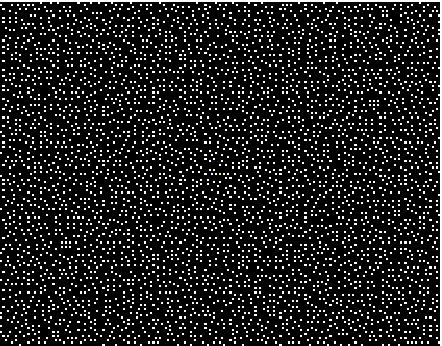
\includegraphics[scale=0.4]{kinect-pattern}}
\\
\uncover<3->{camera\\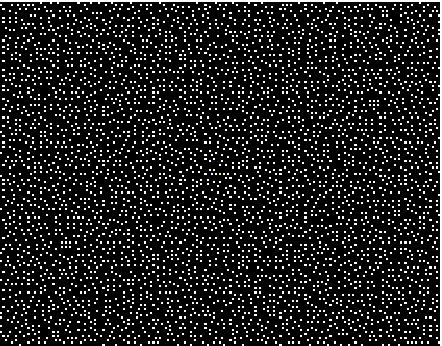
\includegraphics[scale=0.4]{kinect-pattern}}
\end{columns}
\end{frame}


\section{Applicatie}
\subsection{Freenect}
\begin{frame}{Modifications to Freenect}
\begin{itemize}
\item Freenect: opensource driver Kinect
\item Geen infrarood beeld
\item Hack nodig voor calibratie
\end{itemize}
\pause
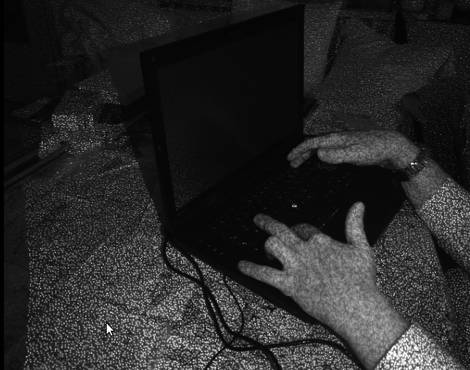
\includegraphics[scale=0.4]{kinect-ir-image.jpg}

\end{frame}
\subsection{Calibratie}


\begin{frame}{Stereo calibratie}
\alt<2->
{
\[
s m' = A \left[R|t\right]M'
\]
or
\[
s 
\left[ \begin{array}{c} 
u\\
v\\
1  
\end{array} \right]
=
\left[ \begin{array}{ccc} 
f_x & 0 & c_x\\
0 & f_y & c_y\\
0 & 0 & 1  
\end{array} \right]
\left[ \begin{array}{cccc}
r_{11} & r_{12} & r_{13} & t_1\\
r_{21} & r_{22} & r_{23} & t_2\\
r_{31} & r_{32} & r_{33} & t_3
\end{array} \right]
\left[ \begin{array}{c} 
X\\
Y\\
Z\\
1  
\end{array} \right]
\]\\
$f_{x},f_{y}$: focal lengths\\
$c_x,c_y$: coordinaten van principal point
}
{
\begin{itemize}
\item Undistort
\item Rectify
\item Translate
\end{itemize}
\centerline{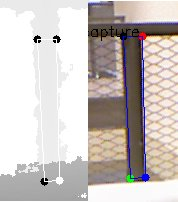
\includegraphics[scale=0.4]{rectify.jpg}}
}
\end{frame}

\begin{frame}{Open CV}
\alt<2->
{
\centerline{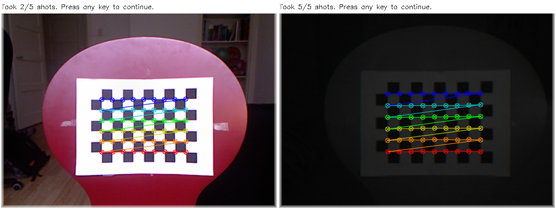
\includegraphics[scale=0.4]{chessboard.png}}
}
{
We gebruiken:
\begin{itemize}
\item \texttt{FindChessboardCorners}
\item \texttt{DrawChessboardCorners}
\item \texttt{StereoCalibrate}
\item \texttt{StereoRectify}
\item \texttt{FindHomography}
\end{itemize}
}
\end{frame}

\begin{frame}{Echte diepte}
Dr. St ́phane Magnenat

\begin{itemize}
\item $depth = 12.36 * tan(rawdepth / 2842.5 + 1.1863)$
\end{itemize}
\end{frame}

\subsection{Model maken}
\begin{frame}{3D model maken}
Eerst:
\begin{itemize}
\item \texttt{InitUndistortRectifyMap}
\item \texttt{WarpPerspective}
\end{itemize}
\end{frame}
\begin{frame}{Extrinsic matrix}
\alt<2->{
\centerline{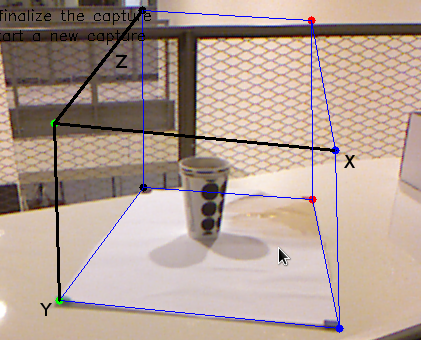
\includegraphics[scale=0.4]{axis.png}}
}
{
Extrinsic matrix met \texttt{FindExtrinsicCameraParams2} en \texttt{Rodriques2}
$$
s \left[ \begin{array}{ccc} 
u\\
v\\
1 \end{array} \right] = 
\left[ \begin{array}{cccc} 
r_{11} & r_{12} & r_{13} & t_{1}\\
r_{21} & r_{22} & r_{23} & t_{2}\\
r_{31} & r_{32} & r_{33} & t_{3} \end{array} \right] 
\left[ \begin{array}{ccc} 
x\\
y\\
z\\
1  \end{array} \right] 
$$
}
\end{frame}
\begin{frame}{De punten verkrijgen}
Bepaal de waarde voor $s$ door $depth(u,v)$.
$$
\left[ \begin{array}{c} 
x\\
y\\
z\end{array} \right] 
=
\left[ \begin{array}{ccc} 
r_{11} & r_{12} & r_{13}\\
r_{21} & r_{22} & r_{23}\\
r_{31} & r_{32} & r_{33}
\end{array} \right]^{-1}
\left[ \begin{array}{c} 
u s\\
v s\\
s \end{array} \right]
-
\left[ \begin{array}{c} 
t_{1}\\
t_{2}\\
t_{3}
\end{array} \right]
$$
\end{frame}
\subsection{PCV}
\begin{frame}{Point cloud viewer}
VPython
\end{frame}
\setbeamercolor{headline}{parent=white}

\begin{frame}

\end{frame}
\setbeamercolor*{headline}{parent=palette primary}
\section{}

\end{document}
